\documentclass{ddis-thesis}
\usepackage{amsmath, amsthm, amssymb}
%\usepackage[latin1]{inputenc}
\usepackage[utf8]{inputenc}
\inputencoding{utf8}
\usepackage{program}
\usepackage{mathrsfs}
\usepackage{amsfonts}
\usepackage{scrextend}
\usepackage{tabularx}
\usepackage{ dsfont }
\usepackage{multirow}


\usepackage{fancyvrb}
\DefineVerbatimEnvironment{code}{Verbatim}{fontsize=\small}
\DefineVerbatimEnvironment{example}{Verbatim}{fontsize=\small}


\usepackage{fancyhdr}% fancyhdr related command; details in its documentation
\pagestyle{fancy}
\fancyhead{}
\fancyhead[LE,RO]{\thepage}
\fancyhead[RE]{\leftmark}
\fancyhead[LO]{\rightmark}

\usepackage{graphicx}
\author{Marco Unternährer}
\title{Heterogeneous Information Sources for Recommender Systems}
\begin{document}



% *************** Front matter ***************

\frontmatter
\begin{titlepage}

\setlength{\textwidth}{16cm}
\setlength{\oddsidemargin}{0cm}
\setlength{\evensidemargin}{0cm}
\setlength{\topmargin}{8mm}
\setlength{\headheight}{0cm}
\setlength{\headsep}{0cm}
\setlength{\topskip}{0cm}
\enlargethispage{5cm}

\noindent
\setlength{\unitlength}{1mm}

\begin{picture}(160,226)
\centering

\put(0,203){\line(1,0){160}} % lower line
\put(109,39){\line(1,0){50}}
\put(109,161){\line(1,0){50}}
\put(109,170){\line(1,0){50}}
\put(107,1){\line(0,1){200}}

\put(0,140){\parbox[b]{100mm}{
    \begin{center}
    {\bf\Huge {\sffamily{Heterogeneous Information Sources for Recommender Systems}}}
    \end{center}}}


\put(109,92){\parbox[b]{50mm}{
    {\bf
    {\sffamily{{\Large Marco Unternährer}}}}\\
    {\sffamily{of Romoos, LU, Switzerland\\\\
    Student-ID: 07-118-771\\
    marco.unternaehrer@uzh.ch
    }}
}}

\put(109,161){\makebox(50,9){{\sffamily{Bachelor Thesis \hfill\today}}}}

\put(0,215){\makebox(80,11)[l]{
\includegraphics[height=2.8cm]
{./section-title/figures/uzh_logo_e_pos}}}


\put(109,32){\parbox[b]{50mm}{\flushleft
		{\sffamily{Advisor:}} {\bf {\sffamily{Bibek Paudel}} }
	}
}

\put(109,10){\parbox[b]{50mm}{\flushleft
        {\sffamily{
        Prof. Abraham Bernstein, PhD\\
        Institut f\"ur Informatik\\
        Universit\"at Z\"urich\\
        http://www.ifi.uzh.ch/ddis}
        }
}}

\end{picture}
\end{titlepage}



\begin{acknowledgements}
I would like to express my gratitude to Prof. Abraham Bernstein for giving me the opportunity to write this thesis.
In particular, I would like to thank my advisor Bibek Paudel for his great effort and patience.
He has guided me well, provided me with many valuable suggestions and carefully reviewed this work.
I am also very grateful for the enduring support throughout my studies of my family and friends.
\end{acknowledgements}

\begin{zusammenfassung}
Der meist angewandte Algorithmus für Empfehlungssysteme basiert auf kollaborativem Filtern, welcher dazu nur die Bewertungen von Objekten durch Benutzer verwendet.
Diese Arbeit präsentiert zwei neue Ansätze wie zusätzliche Daten in Form von Merkmalsvektoren eingesetzt werden können, um bessere Top-N Empfehlungen abzugeben.
Unser erstes Modell, MPCFs-SI, basiert auf einer nichtlinearen Matrix Faktorisierung (MPCFs) und verwendet die zusätzlichen Daten um das Modell zu regularisieren.
Das zweite Modell, MFNN, ist eine Kombination aus Matrix Faktorisierung und einem neuralen Netz und spielt die zusätzlichen Daten als Eingabe ins neurale Netz ein.
Unsere Experimente haben gezeigt, dass MPCFs-SI bessere Leistungen erbringt als das beste Vergleichsmodell MPCFs auf unseren MovieLens 100k und MovieLens 1M Teildatensätzen.
MFNN ist schlechter als das Vergleichsmodell MPCFs auf dem MovieLens 100k Teildatensatz, jedoch ist es auf einem ähnlichen Performanzlevel wie MPCFs-SI auf dem grösseren MovieLens 1M Teildatensatz.
\end{zusammenfassung}

\begin{abstract}
Recommendation systems have become omni-present: we read online news articles, buy books from e-commerce websites and watch videos from online streaming services, which are all very likely to be suggested to us by a recommendation system.
The most common applied algorithm utilizes the collaborative filtering technique, which makes only use of the user-item rating matrix. This thesis introduces two approaches, which make use of extra data about the items.
One of our proposed models, MPCFs-SI, is based on a nonlinear matrix factorization model for collaborative filtering (MPCFs), and uses the extra data to regularize the model.
The second model we propose, MFNN, is an ensemble of a matrix factorization and a neural network and makes direct use of the extra data.
We show that MPCFs-SI slightly outperforms baseline recommender on a subset of both MovieLens 100k and 1M datasets.
Our second model MFNN is always performing worse that the MPCFs model.
\end{abstract}


\tableofcontents

% *************** Main matter ***************
\mainmatter

\chapter{Introduction}
\label{c:introduction}

Recommender systems are software systems suggesting items to users which might fit their personal tastes.
Such systems play a crucial part in e-commerce, social networks, news, music and video websites.

This work investigates methods which make use of data about the users, the items and ratings.

In Chapter \ref{c:incorporating-extra-data} we present two ways of incorporating extra data into recommender systems.
The evaluation of the proposed methods are compared with state-of-the-art methods in Chapter \ref{c:evaluation}.
The first section of this chapter gives an a brief overview over different methods for recommending systems.
We further discuss related work in Section \ref{st:related-work} and conclude this chapter with our motivation for this work.

\section{Background}
\label{st:background}

Methods which try to predict valuable items for a given user can be broadly classified into two groups: collaborative filtering (CF) based methods and content based methods.
These methods differ in what kind of input data they need.
Collaborative filtering methods make use of the user-item rating matrix in order to build models \cite{Kabbur2014}.
Among all the CF algorithms, the most successful ones are the latent factor models \cite{Bao2014}.
These models try to explain user ratings by characterizing both items and users on factors inferred from the rating patterns \cite{Bao2014}.
Content based methods on the other hand make use of meta data about the items as well as the users.
A combination of several methods is referred to as hybrid recommender systems \cite{Ricci2011}.
The purpose of such hybrid systems is to use the advantages of one method and fix the disadvantages of another \cite{Ricci2011}.

While CF techniques are very popular and widely used, one of its main disadvantages is known as the cold start problem \cite{Christoffel2014}.
Collaborative filtering methods require new users to rate some items before the system can suggest items, and new items need to be rated before it can be recommended to users.
In case of the cold start problem, the rating history on a user or item is not sufficient to generalize well to future preferences.
Often though, other sources of information provide richer cues on cold start users or items.


\section{Related Work}
\label{st:related-work}
In this section, we review related approaches to our work.

Simultaneously considering the ratings and the accompanied review text was proposed in \cite{Bao2014}.
The presented model, called \textbf{TopicMF}, learns a recommender model by combining latent factor modeling of rating data with topic modeling in user-review texts.
\cite{Bao2014} show on 22 real-world datasets that their method handles the data sparsity better than state-of-the-art latent factor models.

\cite{Almahairi2015} also have shown that utilizing additional data as a way of regularizing the derived item representations improve the generalization performance of a rating prediction model.
While \cite{Bao2014} have used topic modeling for the user-review text, \cite{Almahairi2015} proposed a distributed bag-of-word approach \textbf{BoWLF} and a recurrent neural network approach \textbf{LMLF} to model the user-review texts.


\section{Motivation}
\label{st:motivation}

As we have discussed in the previous section, recent work has shown that better rating predictions can be obtained by incorporating text-based side information.
Motivated by these recent successes, here we explore alternative approaches to exploiting side information for top-N recommendations.
Specifically, we study how feature vectors extracted from movie subtitles can be used to improve the performance of a latent factor model.

We introduce two approaches to incorporate side information into recommender and compare these to state-of-the-art-based approaches \cite{Kabbur2015,Ning2011,Rendle2009}.
 
\chapter{Incorporating Extra Data into Recommender}
\label{c:incorporating-extra-data}


\newcommand{\norm}[1]{\ensuremath{\lVert{#1}\rVert}}
\newcommand{\Abf}[1]{\ensuremath{\mathbf{#1}}}

In this work, we focus particularly on nonlinear methods for collaborative filtering.
After giving an overview of the used notation in the first section, we show a recently developed nonlinear matrix factorization technique proposed in \cite{Kabbur2015} (Section \ref{st:mpcf}), then Section \ref{st:using-extra-data} introduces two models which make use of extra data.


\section{Notation}
\label{st:notation}

As in \cite{Kabbur2015}, all vectors are represented by bold lower case letters (e.g. $\Abf{a}$), all matrices are represented by bold upper case letters (e.g. $\Abf{A}$) and predicted values are denoted by having a $\hat{}$ (hat) over it (e.g. $\hat{a}$).
All important symbols and definitions used in this work are summarized in Table \ref{tab:symbols}.

\begin{table}[p]
	\begin{center}
		\begin{tabularx}{\linewidth}{cX}
			\hline \hline \textbf{Symbol} & \textbf{Definition} \\
			\textit{u, i} & Individual user \textit{u}, item \textit{i} \\
			\textit{n, m} & Number of users and items \\
			\textit{k} & Number of latent factors \\
			\textit{T} & Number of user local preferences \\
			$\mathit{r_{ui}}$ & Rating by user \textit{u} on item \textit{i}\\
			$\mathit{\hat{r}_{ui}}$ & Predicted rating for user \textit{u} on item \textit{i} \\
			\textbf{R} & User-item rating matrix, $\mathbf{R} \in \mathds{R}^{n \times m}$ \\
			\textbf{P} & User latent factor matrix, $\mathbf{P} \in \mathds{R}^{n \times k}$ \\
			\textbf{Q} & Item latent factor matrix, $\mathbf{Q} \in \mathds{R}^{m \times k}$ \\
			\textbf{S} & User latent factor tensor, $\mathbf{S} \in \mathds{R}^{n \times k \times T}$ \\
			$\mathbf{B_u}$ & User-Interest bias matrix, $\mathbf{B_u} \in \mathds{R}^{n \times T}$ \\
			$\mathbf{b_i}$ & Item bias vector, $\mathbf{b_i} \in \mathds{R}^{m}$ \\ 
			$\lambda_{reg}$ & $l_2$-regularization constant\\
			\\
			
			\textit{d} & Number of Doc2Vec dimensions \\
			$\mathbf{f}_i$ & Doc2Vec vector for item \textit{i}, $\mathbf{f}_i \in \mathds{R}^{d}$ \\
			$\mathbf{\hat{f}}_i$ & Predicted Doc2Vec vector, $\mathbf{\hat{f}}_i \in \mathds{R}^{d}$\\
			\textbf{G} & Weight matrix of the Doc2Vec prediction model, $\mathbf{G} \in \mathds{R}^{d \times k}$ \\
			\textbf{h} & Bias vector of the Doc2Vec prediction model, $\mathbf{h} \in \mathds{R}^{d}$ \\
			$\lambda_{ed}$ & Parameter that balances matrix factorization model and the Doc2Vec prediction model \\
			$\lambda_{cos}$ & Parameter that balances the Euclidean and the cosine distance \\
			\\
			
			$\mathbf{w}, \mathbf{W^\prime}$ & Weight vector and matrix of the neural network \\
			$\mathbf{x}$ & Input vector to the neural network, $\mathbf{x} \in \mathds{R}^{2k + d}$ \\
			$\varphi(x)$ & Activation function of the neural network \\
			\hline \hline
		\end{tabularx}
	\end{center}
	\caption{Symbols used and definitions}
	\label{tab:symbols}
\end{table}

\section{Nonlinear Matrix Factorization for Collaborative Filtering}
\label{st:mpcf}

Nonlinear methods make less a priori assumptions on how components of a system may interact \cite{Carello2005}.
A recently developed nonlinear method for top-N recommendation is called \textbf{MaxMF} \cite{Weston2013}.
MaxMF extends the matrix factorization based approaches by representing a user with multiple latent vectors, each corresponding to a different "taste" associated with the user \cite{Kabbur2015}.
These different tastes associated with each user representation are termed as \textit{interests} \cite{Kabbur2015}.
The assumption behind this approach is that it helps to capture user preferences better, especially when the user's interests are diverse \cite{Kabbur2015}.

\cite{Kabbur2015} developed a nonlinear matrix factorization method called \textbf{MPCF}, which is based on MaxMF.
While MaxMF assumes that interest-specific preferences of the users are completely different, MPCF models the user as a combination of global preference and interest-specific latent factors \cite{Kabbur2015}.
In the work of \cite{Kabbur2015}, given a user \textit{u}, an item \textit{i} and \textit{T} user local preferences, the estimated rating \textit{$\hat{r}_{ui}$} is given by the sum of the estimations from global preference and interest-specific preference components.
That is,
\begin{equation}
\hat{r}_{ui} = \mu + b_i + \textbf{p}_u \textbf{q}_i^\intercal + \max_{t=1,..,T} (b_{ut} + f(u, i, t)),
\end{equation}
where $\mu$ is the global bias i.e., the average rating value of the entire data set, $b_i$ is the item bias corresponding to item \textit{i}, $b_{ut}$ is the user-local preference bias corresponding to user \textit{u} and local preference \textit{t}, $\textbf{p}_u$ is the latent vector associated with user \textit{u} and $\textbf{q}_i$ is the latent vector associated with item \textit{i} \cite{Kabbur2015}.
\cite{Kabbur2015} proposed two different methods to represent the interest-specific preference component \textit{f(u, i, t)}.
The first one, named \textbf{MPCFi}, has independent item factors in \textit{f(u, i, t)} compared to that of global preference component, whereas the second one shares the item factors of \textit{f(u, i, t)} with the global preference component, and thus named \textbf{MPCFs}.
The local preference component \textit{f(u, i, t)} for MPCFs is given by,
\begin{equation}
f(u, i, t) = \textbf{s}_{ut} \textbf{q}_i^\intercal,
\end{equation}
where $\textbf{s}_{ut}$ is the user latent vector for \textit{u} in the local preference component corresponding to the local preference \textit{t} and $\textbf{q}_i^\intercal$ is the shared item latent vector between the global preference and the local preference components \cite{Kabbur2015}.
The following regularized optimization problem is minimized to learn \textbf{P}, \textbf{Q}, \textbf{S}, $\mathbf{B_u}$ and $\mathbf{b_i}$ matrices and vectors:
\begin{equation}
\mathcal{L}_{rating} = \frac{1}{2} \sum_{u,i \in R} (r_{ui} - \hat{r}_{ui})^2 + \frac{\lambda_{reg}}{2} (\norm{\Abf{P}}_F^2 + \norm{\Abf{Q}}_F^2 + \norm{\Abf{S}}_F^2 + \norm{\Abf{B_u}}_F^2 + \norm{\Abf{b_i}}_2^2),\label{eq:mpcf-rating}
\end{equation}
where $r_{ui}$ is the ground truth value,  $\hat{r}_{ui}$ is the estimated value, $\mathbf{b_i}$ is the vector corresponding to the item biases, $\mathbf{B_u}$ is the matrix corresponding to the local preference user biases and $\lambda_{reg}$ is the $l_2$-regularization constant for latent factor matrices \cite{Kabbur2015}.
\cite{Kabbur2015} propose to solve the optimization problem in Eq. \ref{eq:mpcf-rating} using a stochastic gradient descent algorithm and provide pseudocode for that.


 

\section{Using Extra Data}
\label{st:using-extra-data}
In this section, we discuss how feature vectors were extracted from movie subtitles, then two approaches are propose to incorporate such vectors in order to improve top-N recommendations.

\subsection{Feature Extraction from Movie Subtitles}
\label{sst:feature-extraction}
Movie subtitles have been from a website called Opensubtitles\footnote{Opensubtitles - http://opensubtitles.org}.
Note that not all subtitles belong to the movies the website has claimed, however, due to the limitation of time, a proper analysis on how many selections were affected and finding solutions were not carried out.
Next, a pre-processing step was removing all non-alphanumerical characters which gave a natural language document per subtitle with an average of 7521 words per document.
With the help of a library called NLTK\footnote{\label{fn:nltk}NLTK - http://www.nltk.org/}, each document was tokenized and stop words were removed.
Gensim\footnote{Gensim - https://radimrehurek.com/gensim/}, a topic modeling library, was then used to generate a feature vector per document via a deep learning algorithm called Paragraph Vectors (also known as Doc2Vec) introduced in \cite{Le2014a}.
The distributed-bag-of-words variant of the Paragraph Vector algorithm and negative sampling was used.
In preliminary experiments, we have tested several Doc2Vec vector dimensions $d$.
While some work on sentiment analysis of movie reviews use 100 dimensions \cite{Qiu2015} or 300 dimensions \cite{Chapman2014}, we have found that a vector size of 50 resulted in higher similarities between movies and their sequels.
The full parameter set is listed in Appendix \ref{a:doc2vec}.
We refer the readers to the excellent notes of \cite{Rong} and \cite{Goldberg2014} to explain in detail how Word2Vec, the common name of the base algorithm of Paragraph Vectors, works.

\subsection{MPCFs-SI: Regularizing with Extra Data}
\label{sst:mpcfs-si}

As discussed in Section \ref{st:related-work}, \cite{Almahairi2015} has shown that utilizing additional data as a way of regularizing the derived item representations has improved the generalization performance of a rating prediction model.
It has accomplished to reduce overfitting by simultaneously estimating the parameters of the matrix factorization to perform well on another related task \cite{Almahairi2015}.
In a similar fashion, we propose to optimize a nonlinear matrix factorization model MPCFs in Eq. \ref{eq:mpcf-rating} and regularize it with a model which predicts the Doc2Vec vector of an item $\mathbf{f}_i$, given the latent vector for that item $\mathbf{q}_i$.
The Doc2Vec prediction is modeled as a simple affine transformation of the item latent vector, as shown in Eq.(\ref{eq:affine-transformation}):

\begin{equation}
\hat{\Abf{f}}_{i} = \Abf{G} \Abf{q}_i + \Abf{h} \label{eq:affine-transformation},
\end{equation}
where $\hat{\Abf{f}}_i$ is the predicted Doc2Vec vector for item $i$, $\Abf{G}$ and $\Abf{h}$ are a weight matrix and a bias vector to be learned.
Since we are transforming from one vector space into another, we have decided to use the squared Euclidean and cosine distances as part of the loss term.
We can informally think of minimizing the Euclidean distance as preserving the magnitude of the vector, while minimizing the cosine distance helps with the vector direction. 
Therefore, the loss term for the Doc2Vec prediction model is given in Eq. \ref{eq:ed-loss}:
\begin{equation}
\mathcal{L}_{ed} = \sum_{u,i \in R} (\norm{\Abf{f}_i - \hat{\Abf{f}}_i}_F^2 + \lambda_{cos} D_C(\Abf{f}_i, \hat{\Abf{f}}_i)) + \lambda_{reg} \norm{\Abf{G}}_F^2  \label{eq:ed-loss},
\end{equation}
where $\Abf{f}_i$ is a Doc2Vec vector for item $i$ extracted from movie subtitles via deep learning methods discussed in the previous section, $\lambda_{cos}$ is a parameter that balances the performance of the squared Euclidean distance and the cosine distance, $D_C(\Abf{f}_i, \hat{\Abf{f}}_i)$ is the cosine distance and $\lambda_{reg}$ is the $l_2$-regularization constant for the weight matrix.
The cosine similarity $S_C$ and the cosine distance $D_C$ between two vectors $\Abf{a}$ and $\Abf{b}$ are defined as,
\begin{align}
	S_C(\Abf{a}, \Abf{b}) = \frac{\Abf{a} \cdot \Abf{b}}{\norm{\Abf{a}} \norm{\Abf{b}}} \in [-1, 1], \label{eq:cosine-sim}\\
	D_C(\Abf{a}, \Abf{b}) = 1 - S_C(\Abf{a}, \Abf{b}) \in [0, 2],
\end{align}
where $\norm{\Abf{a}}$ is the length of the vector $\Abf{a}$.
A cosine similarity between two vectors $\Abf{a}$ and $\Abf{b}$ is 1, if they point exactly in the same direction in the vector space, while a value of 0 means that the vectors are orthogonal and a value of -1 means that they point in the exact opposite direction in the vector space.

We have also considered modeling the Doc2Vec prediction with a neural network.
Preliminary results have shown that a neural network model does not improve our main measure AUC.

%\begin{figure}[p]
%	\centering
%	\includegraphics[width=0.5\linewidth]{./section-chapter1/figures/mpcf-si-nn.pdf}
%	\caption[MPCFs-SI: Feature Prediction Model As A Neural Network]
%	{MPCFs-SI: Feature Prediction Model As A Neural Network}
%	\label{f:mpcfs-si-nn}
%\end{figure}

We propose to linearly combine the matrix factorization with the Doc2Vec prediction model.
Therefore, the full loss term to minimize is the following:
\begin{equation}
\begin{aligned}
	\mathcal{L} &= \mathcal{L}_{rating} + \lambda_{ed} \mathcal{L}_{ed} \\
				&= \frac{1}{2} \sum_{u,i \in R} (r_{ui} - \hat{r}_{ui})^2 + \frac{\lambda_{reg}}{2} (\norm{\Abf{P}}_F^2 + \norm{\Abf{Q}}_F^2 + \norm{\Abf{S}}_F^2 + \norm{\Abf{B_u}}_F^2 + \norm{\Abf{b_i}}_2^2) \\
				& + \lambda_{ed} (\sum_{u,i \in R} (\norm{\Abf{f}_i - \hat{\Abf{f}}_i}_F^2 + \lambda_{cos} D_C(\Abf{f}_i, \hat{\Abf{f}}_i)) + \lambda_{reg} \norm{\Abf{G}}_F^2),
\end{aligned}
\end{equation}
where $\lambda_{ed}$ is a parameter that balances the performance of the matrix factorization model and the Doc2Vec prediction model, which was one of the parameters to be determined by running grid search.


We apply AdaGrad, a stochastic gradient descent variant, to update $\mu, \Abf{P}, \Abf{Q}, \Abf{S}, \Abf{B_u}$ and $\Abf{b_i}$.
The gradients for the matrix factorization model are directly from \cite{Kabbur2015}.
We have implemented the Doc2Vec prediction model in Theano and update $\Abf{G}$ and $\Abf{h}$ with AdaGrad as well.
Theano offers automatic differentiation such that we simply add $\lambda_{ed} \frac{\partial \mathcal{L}_{ed}}{\partial \Abf{q}_i}$ to the item factor gradient $\frac{\partial \mathcal{L}_{rating}}{\partial \Abf{q}_i}$.

As \cite{Kabbur2015} suggested, gradient updates for model parameters are computed for both rated and non-rated entries of $\mathbf{R}$, which is a common practice for the top-N recommendation task.
We sample zero entries corresponding to non-rated items on every epoch and add these to the actual training ratings.
\cite{Kabbur2015} indicates that the ratio between rated and non-rated within the range of 1:3 to 1:5 is sufficient to produce the best model.

%The corresponding gradients are as follows:
%
%\begin{equation}
%\begin{aligned}
%-1 \cdot \frac{\partial \mathcal{L}}{\partial b_i} &= (r_{ui} - \hat{r}_{ui}) - \lambda_{reg} b_i \\
%-1 \cdot \frac{\partial \mathcal{L}}{\partial b_{ut^*}} &= (r_{ui} - \hat{r}_{ui}) - \lambda_{reg} b_{ut^*} \\
%-1 \cdot \frac{\partial \mathcal{L}}{\partial \Abf{p}_u} &= (r_{ui} - \hat{r}_{ui}) \Abf{q}_i - \lambda_{reg} \Abf{p}_u \\
%-1 \cdot \frac{\partial \mathcal{L}}{\partial \Abf{q}_i} &= (r_{ui} - \hat{r}_{ui}) (\Abf{p}_u + \Abf{w_{ut^*}}) + \lambda_{ed} ((\Abf{f}_i - \hat{\Abf{f}}_i) \cdot \Abf{G})^\intercal - \lambda_{reg} \Abf{q}_i \\
%-1 \cdot \frac{\partial \mathcal{L}}{\partial \Abf{s}_{ut^*}} &= (r_{ui} - \hat{r}_{ui}) \Abf{q}_i - \lambda_{reg} \Abf{s}_{ut^*} \\
%-1 \cdot \frac{\partial \mathcal{L}}{\partial \Abf{G}} &= \lambda_{ed} (\Abf{f}_i - \hat{\Abf{f}}_i) \cdot \Abf{q}_i - \lambda_{reg} \Abf{G} \\
%-1 \cdot \frac{\partial \mathcal{L}}{\partial \Abf{h}} &= \lambda_{ed} (\Abf{f}_i - \hat{\Abf{f}}_i)
%\end{aligned}
%\end{equation}
%where $t^*$ is the local preference corresponding to maximum score of the local preference component.

When we use the introduced Doc2Vec prediction model together with the nonlinear matrix factorization model MPCFs, we call this joint model \textbf{MPCFs-SI}.

\newpage
\subsection{MFNN: Neural Network}
\label{sst:mfnn}

The second model is an ensemble of a matrix factorization model and a neural network model.
This model is called \textbf{MFNN}.
Inspired by the MPCFs model, it has the ability to incorporate additional user or item data directly as an input to the neural network.
As in MPCFs, the matrix factorization is used to model a global preference, while a nonlinear method is used to model local preferences.

The estimated rating \textit{$\hat{r}_{ui}$} is given by:

\begin{align}
	\hat{r}_{ui} &= \mu + b_i + \textbf{p}_u \textbf{q}_i^\intercal + nn(u, i),
\end{align}
where $\mu$ is the global bias, $b_i$ is the item bias corresponding to item \textit{i}, $\textbf{p}_u$ is the latent vector associated with user \textit{u}, $\textbf{q}_i$ is the latent vector associated with item \textit{i} and $nn(u, i)$ is a user-item specific local preference component.
The user-item specific local preference component $nn(u, i)$ is defined as,
\begin{align}
	nn(u, i) &= \sum_{j=1}^{J} (w_{j} \varphi(\sum_{l=1}^{L} w^\prime_{j,l} x_l)),\\
	\mathbf{x} &= (\mathbf{p}_u, \mathbf{q}_i, \mathbf{f}_i), \\
	\varphi(x) &= \max(0, x),
\end{align}
where $w_{\cdot}$ and $w_{\cdot,\cdot}^\prime$ are weights of the neural network model to be learned, $\mathbf{x}$ is a concatenation of the user latent vector $\mathbf{p}_u$, the item latent vector $\mathbf{q}_i$ and the side information as a Doc2Vec vector $\mathbf{f}_i$, $J$ is the number of neurons in the hidden layer, $L$ is the length of $\mathbf{x}$ and $\varphi(x)$ is the activation function.
$J$, the number of neurons in the hidden layer, is somewhat related to $T$, the number of user local preferences in the MPCF model.
Modeling user-item specific local preferences as a neural network enables the interaction of these local preferences, whereas in MPCF the user local preferences are independent and do not interact.
Figure \ref{f:mfnn} shows the neural network in a diagram.

The loss term to minimize for this model is as follows:
\begin{equation}
\begin{aligned}
\mathcal{L} &= \frac{1}{2} \sum_{u,i \in R} (r_{ui} - \hat{r}_{ui})^2 + \frac{\lambda_{reg}}{2} (\norm{\Abf{P}}_F^2 + \norm{\Abf{Q}}_F^2 + \norm{\Abf{b_i}}_2^2) + \frac{\lambda_{nn reg}}{2}(\norm{\Abf{w}}_2^2 + \norm{\Abf{W^\prime}}_F^2)\\
\end{aligned}
\end{equation}

Like in the previous model MPCFs-SI, we apply AdaGrad to update $\mu, \Abf{P}, \Abf{Q},$ and $\Abf{b_i}$.
The neural network was implemented in Theano and we also use AdaGrad to update its parameters $\Abf{w}$ and  $\Abf{W^\prime}$.
The sampling of non-rated items is done the same way as in our first model.

\begin{figure}[p]
	\centering
	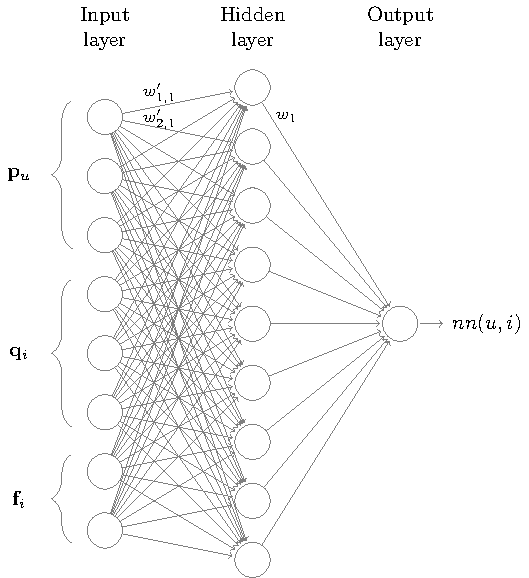
\includegraphics[width=0.7\linewidth]{./section-chapter1/figures/mfnn.pdf}
	\caption[MFNN: Neural Network]
	{MFNN: Neural Network}
	\label{f:mfnn}
\end{figure}


\chapter{Evaluation}
\label{c:evaluation}

In the previous chapter, we introduced two approaches, MPCFs-SI and MFNN, to incorporate side information into the recommender.
The first section of this chapter gives an overview of the used datasets (Section \ref{st:datasets}), followed by the baseline recommender (Section \ref{st:baseline}) and the evaluation methodology (Section \ref{st:methodology}).
We then state which performance measures were calculated (Section \ref{st:performance-measures}).
Section \ref{st:performance-comparison} shows how the proposed models perform compared to state-of-the-art models.
We conclude this chapter with an outline of our software setup in Section \ref{st:system-setup}.

\section{Datasets}
\label{st:datasets}
Our datasets are based on the MovieLens 100k and the MovieLens 1M datasets\footnote{MovieLens Datasets - http://grouplens.org/datasets/movielens/} and call them ML-100k-sub and ML-1M-sub respectively.
Only movie ratings were selected based on whether or not their respective movie subtitle was found.
Subtitles were downloaded from Opensubtitles\footnote{Opensubtitles - http://opensubtitles.org}.
The datasets have rating values from 1 to 5.
Converting the ratings into implicit feedback by setting the positive ratings to 1 was applied as it is commonly done for the top-N recommendation task \cite{Kabbur2015}.
Table \ref{tab:datasets} shows the number of ratings and movies that were selected in the subsets.
The rank-size distributions, explaining how many times each movie has been rated and ranked by that value, are presented in Figures \ref{f:ml-100k-tail} and \ref{f:ml-1m-tail}.
An analysis of the rank-size distribution has shown that the ML-100k-sub dataset, in particular, has lost a bit of its tail.

\begin{table}[h]
	\begin{center}
		\begin{tabularx}{\linewidth}{Xccc}
			\hline \hline
			\textbf{Dataset} & \textbf{\# Ratings} & \textbf{\# Movies} & \textbf{\# Users} \\
			MovieLens 100k & 100'000 & 1682 & 943 \\
			ML-100k-sub & 91'178 & 1261 & 943 \\
			MovieLens 1M & 1'000'000 & 3883 & 6040 \\
			ML-1M-sub & 978'026 & 3005 & 6040 \\
			\hline \hline
		\end{tabularx}
	\end{center}
	\caption{Datasets}
	\label{tab:datasets}
\end{table}

\begin{figure}[p]
	\centering
	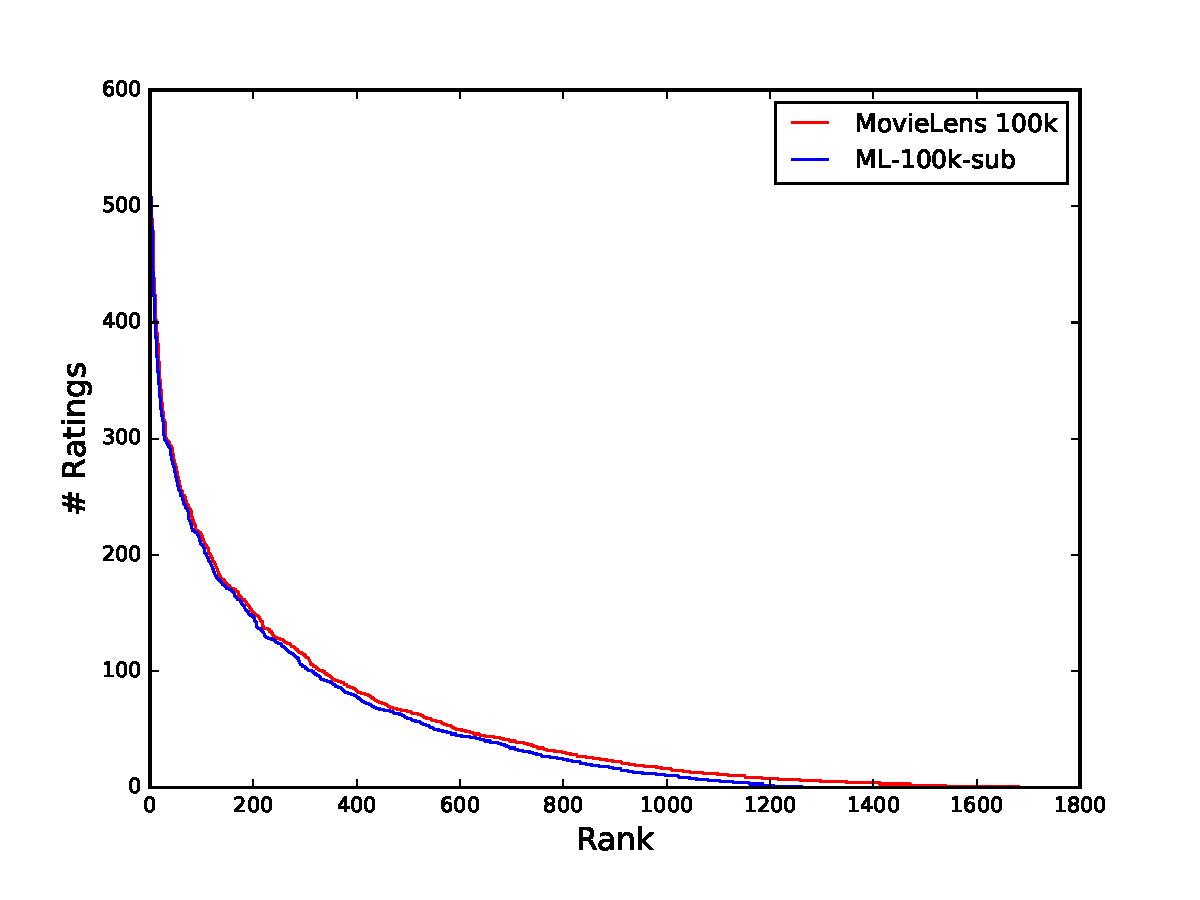
\includegraphics[width=0.7\linewidth]{./section-chapter2/figures/ml-100k_tail.pdf}
	\caption{Rank-size distribution of the MovieLens 100k and ML-100k-sub datasets}
	\label{f:ml-100k-tail}
\end{figure}

\begin{figure}[p]
	\centering
	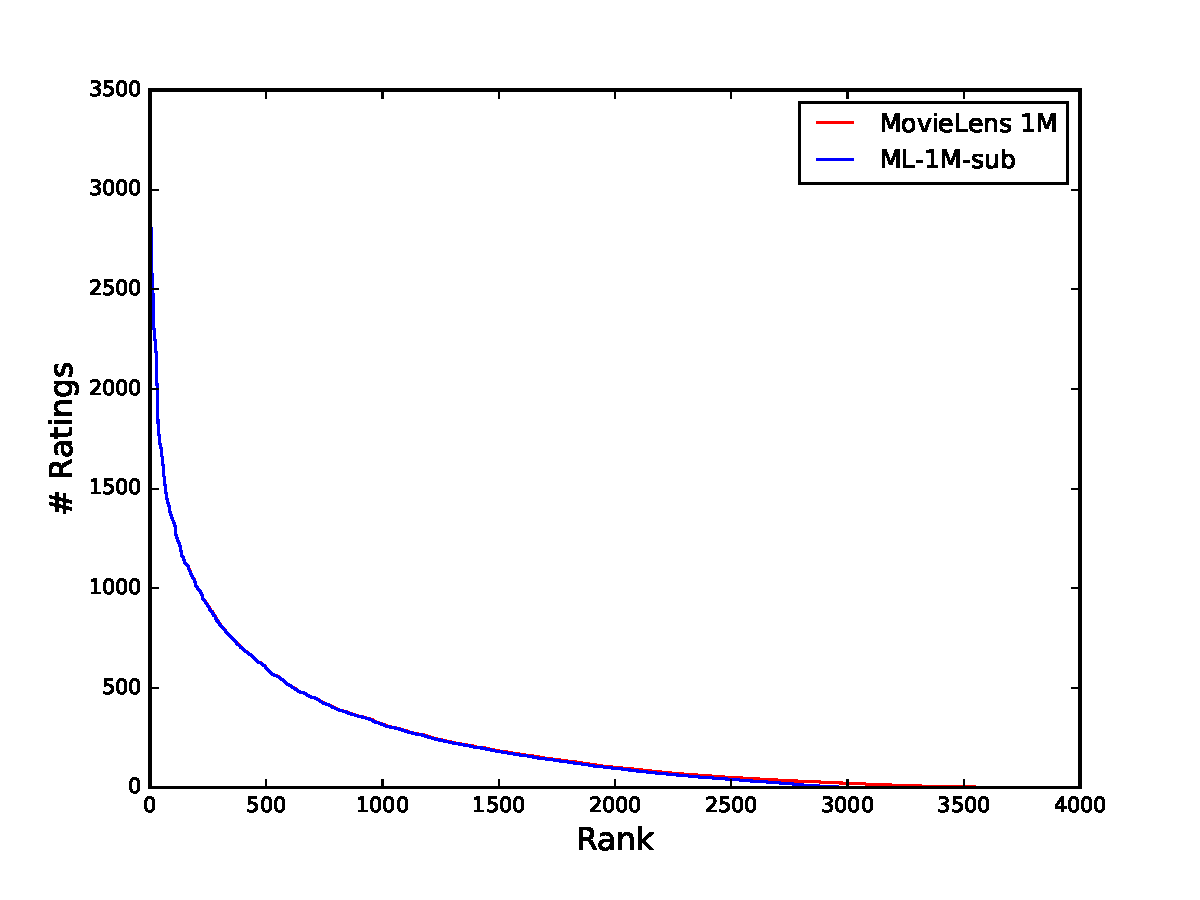
\includegraphics[width=0.7\linewidth]{./section-chapter2/figures/ml-1m_tail.pdf}
	\caption{Rank-size distribution of the MovieLens 1M and ML-1M-sub datasets}
	\label{f:ml-1m-tail}
\end{figure}

\section{Baseline}
\label{st:baseline}

Both the MPCFs-SI (Section \ref{sst:mpcfs-si}) and MFNN (Section \ref{sst:mfnn}) models were compared against three baseline methods.
The baseline recommender consists of the nonlinear matrix factorization model MPCFs discussed in Section \ref{st:mpcf}, a linear recommender called SLIM \cite{Ning2011}, and another state-of-the-art recommender also based on a latent factor model obtained with matrix factorization, called BPRMF \cite{Rendle2009}.

\section{Methodology}
\label{st:methodology}
The standard way of splitting datasets for evaluating recommendation systems is that a percentage of each user's ratings remain in the training set while the rest goes into the test set.
However, datasets have been subdivided, such that 70\% of each movie's ratings were used for training, and the rest for testing.
The rational explanation of this method of splitting the sample is to make the movie data especially sparse.
We were also making sure that each user has at least one rating in the test set in order to measure the performance.

For each recommender, a parameter grid was defined and 12 or more parameter sets were randomly drawn from that grid.
The parameter set which resulted in the best area under the ROC curve (AUC) for each model was then selected.
The best parameter sets are listed in Appendix \ref{a:best-params}.
The performance of the methods was then evaluated using five different randomly drawn splits in a manner described in the previous paragraph.

Measures were reported after 20 iterations for MPCFs, MPCFs-SI, and BPRMF.
The number of iterations for the SLIM model was a hyperparameter.
We have found that five epochs give us the best results.
Our model MFNN is computationally quite expensive and takes a lot of time.
We also ran 20 iterations of the MFNN model on the ML-100k-sub, however, we had to limit the number of iterations of that model for the ML-1M-sub dataset to 10 epochs.

\section{Performance Measures}
\label{st:performance-measures}
We use the area under the ROC curve (AUC) as our main measure to evaluate each approach.
Moreover, we have adopted several commonly used measures to evaluate the performance of the recommender.
The following measures were calculated: area under the ROC curve (AUC), Precision@20 (P@20), Recall@20 (R@20), Mean Reciprocal Rank (MRR) and Spearman Rank Correlation (SRC).
Furthermore, we have carried out an additional measure related to AUC: Instead of recommending items to users and calculate the ranking measure, we were recommending users to items and calculating the rank measure for each item.
This is called IAUC.


\section{Performance Comparison}
\label{st:performance-comparison}


Measures were defined in Section \ref{st:performance-measures} and used to determine the performance of the models introduced in Section \ref{st:using-extra-data} as well as the baseline recommender.
MPCFs-SI performs better on all calculated performance measures on ML-100k-sub compared to the best baseline recommender, which is MPCFs.
On ML-1M-sub, MPCFs-SI is superior to MPCFs in terms of AUC, IAUC and Spearman Rank Correlation.
Results show that MFNN is inferior to \text{MPCFs} on all measures except Precision@20 and Recall@20 on the ML-100k-sub dataset.
MFNN is performing at a similar level as MPCFs-SI regarding AUC and has the best Spearman Rank Correlation of all recommender on the bigger ML-1M-sub.
The full results are summarized in Table \ref{tab:performance}.

Table \ref{tab:item-factor-sim} presents that similar movies have a high cosine similarity (defined in Eq. \ref{eq:cosine-sim}) in the document vector space.
In fact, the sequels to the listed movies were the most or second most similar movie in that space.
Moreover, looking at the item latent vector space, results show that using MPCFs-SI improves the cosine similarity of all similar items compared to using MPCFs.
The most dissimilar movies in the document vector space of the first listed movies are also analyzed.
MPCFs-SI also separates dissimilars apart and thus decreases the cosine similarity of those movies.
MFNN seems to make all listed movies more similar, irregardless of them being similar in the document vector space or not.
The best performing models on the ML-1M-sub dataset were used to calculate the cosine similarities in Table \ref{tab:item-factor-sim}.

One of our goals was also addressing the cold-start problem.
Our hypothesis here is that incorporating side information would lead to better recommendations for users who have very few ratings.
Figures \ref{f:ml-100k-comp-auc} (ML-100k-sub dataset) and \ref{f:ml-1m-comp-auc} (ML-1M-sub dataset) show the average AUC for a group of users as users with more training ratings were included into that group.

It is surprising that the average AUC goes down the more users with many training ratings are being included in Figure \ref{f:ml-100k-comp-auc}.
However, this must be caused by an inherent characteristic of the ML-100k-sub dataset as that trend is seen for all recommender.
We do not observe that using MPCFs-SI or MFNN improve the AUC for users who have very few ratings on the ML-100k-sub dataset.

On the bigger ML-1M-sub dataset, Figure \ref{f:ml-1m-comp-auc} and Figure \ref{f:ml-1m-comp-auc-zoom} (the zoomed version thereof) indicate that the MFNN model is superior to the other recommender in terms of AUC for users with less than 200 training ratings in particular.
However, MPCFs-SI seems to have an advantage for users with less than 10 training ratings.

For the sake of completeness, the progressions of the average of the other defined measures are presented in Figures \ref{f:ml-100k-comp-iauc} and \ref{f:ml-100k-comp-group} for the ML-100k-sub dataset, and in Figures \ref{f:ml-1m-comp-iauc} and \ref{f:ml-1m-comp-group} for the ML-1M-sub dataset.
\begin{table}[p]
	\begin{center}
		\begin{tabularx}{\linewidth}{cXcccccc}
			\hline \hline
			& \textbf{Method} & \textbf{AUC} & \textbf{IAUC} & \textbf{P@20} & \textbf{R@20} & \textbf{MRR} & \textbf{SRC}\\
			\hline
			\parbox[t]{2mm}{\multirow{7}{*}{\rotatebox[origin=c]{90}{ML-100k-sub}}} & Perfect & 100.0 & 100.0 & 100.0 & 100.0 & 1.0 & 1.0\\
			& MPCFs-SI & \textbf{93.76} & \textbf{90.83} & 28.16 & \textbf{44.27} & \textbf{0.6866} & \textbf{0.2005}\\
			& MFNN & 93.48 & 89.74 & \textbf{28.44} & 43.96 & 0.6741 & 0.1925 \\
			& \multicolumn{7}{c}{\hdashrule[0.5ex][c]{14cm}{0.5pt}{1mm}} \\
			& MPCFs & 93.65 & 90.78 & 27.79 & 43.55 & 0.6770 & 0.1974 \\
			& BPRMF & 92.20 & 68.03 & 18.00 & 27.38 & 0.3703 & 0.1567 \\
			& SLIM & 91.45 & 85.20 & 23.49 & 37.75 & 0.5993 & 0.1880 \\
			\hline
			\parbox[t]{2mm}{\multirow{7}{*}{\rotatebox[origin=c]{90}{ML-1M-sub}}} & Perfect & 100.0 & 100.0 & 100.0 & 100.0 & 1.0 & 1.0\\
			& MPCFs-SI & 92.88 & \textbf{92.15} & 32.11 & 32.77 & 0.6941 & 0.2260 \\
			& MFNN & \textbf{92.89} & 91.73 & 30.36 & 29.54 & 0.6481 & \textbf{0.2351} \\
			& \multicolumn{7}{c}{\hdashrule[0.5ex][c]{14cm}{0.5pt}{1mm}} \\
			& MPCFs & 92.81 & 92.08 & \textbf{32.71} & \textbf{33.44} & \textbf{0.7035} & 0.2223 \\
			& BPRMF & 91.82 & 67.54 & 21.23 & 20.13 & 0.4430 & 0.2013 \\
			& SLIM & 91.23 & 88.00 & 28.59 & 28.76 & 0.6465 &  0.2322 \\
			\hline \hline
		\end{tabularx}
	\end{center}
	\caption{Performance measures. The best result for each measure and dataset is highlighted in bold.}
	\label{tab:performance}
\end{table}


\begin{table}[p]
	\begin{center}
		\begin{tabularx}{\linewidth}{XXcccc}
			\hline \hline
			\textbf{Movie 1} & \textbf{Movie 2} & \textbf{Doc2Vec} & \textbf{MPCFs} & \textbf{MPCFs-SI} & \textbf{MFNN} \\
			\hline
			Free Willy & Free Willy 2 & 0.8694 & 0.6915 & 0.7329 & 0.8305\\
			Jurassic Park & Jurassic Park 2 & 0.6796 & 0.5418 & 0.6214 & 0.7440\\
			Scream & Scream 2 & 0.7514 & 0.7016 & 0.7362 & 0.8325\\
			Species & Species II & 0.6831 & 0.6641 & 0.7015 & 0.8203\\
			Star Wars V & Star Wars VI & 0.9231 & 0.6846 & 0.7650 & 0.8717\\
			Toy Story & Toy Story 2 & 0.7529 & 0.6546 & 0.6838 & 0.7929\\
			\hline
			Free Willy & Mrs. Brown & -0.0141 & -0.0366 & -0.0927 & 0.0977\\
			Jurassic Park & Battling Butler & -0.1127 & -0.1218 & -0.1805 & -0.0083\\
			Scream & Kelly's Heroes & -0.0465 & -0.1385 & -0.1971 & -0.0868\\
			Species & Patton & -0.0763 & -0.0283 & -0.0485 & 0.0942\\
			Star Wars V & Angela's Ashes & -0.0130 & -0.1433 & -0.1732 & -0.1183\\
			Toy Story & Raise the Red Lantern & -0.0257 & -0.0256 & -0.0490 & 0.0593\\
			\hline \hline
		\end{tabularx}
	\end{center}
	\caption{Item cosine similarities, measured in the document vector space and the item latent vector space of the according model.}
	\label{tab:item-factor-sim}
\end{table}


\begin{figure}[p]
	\centering
	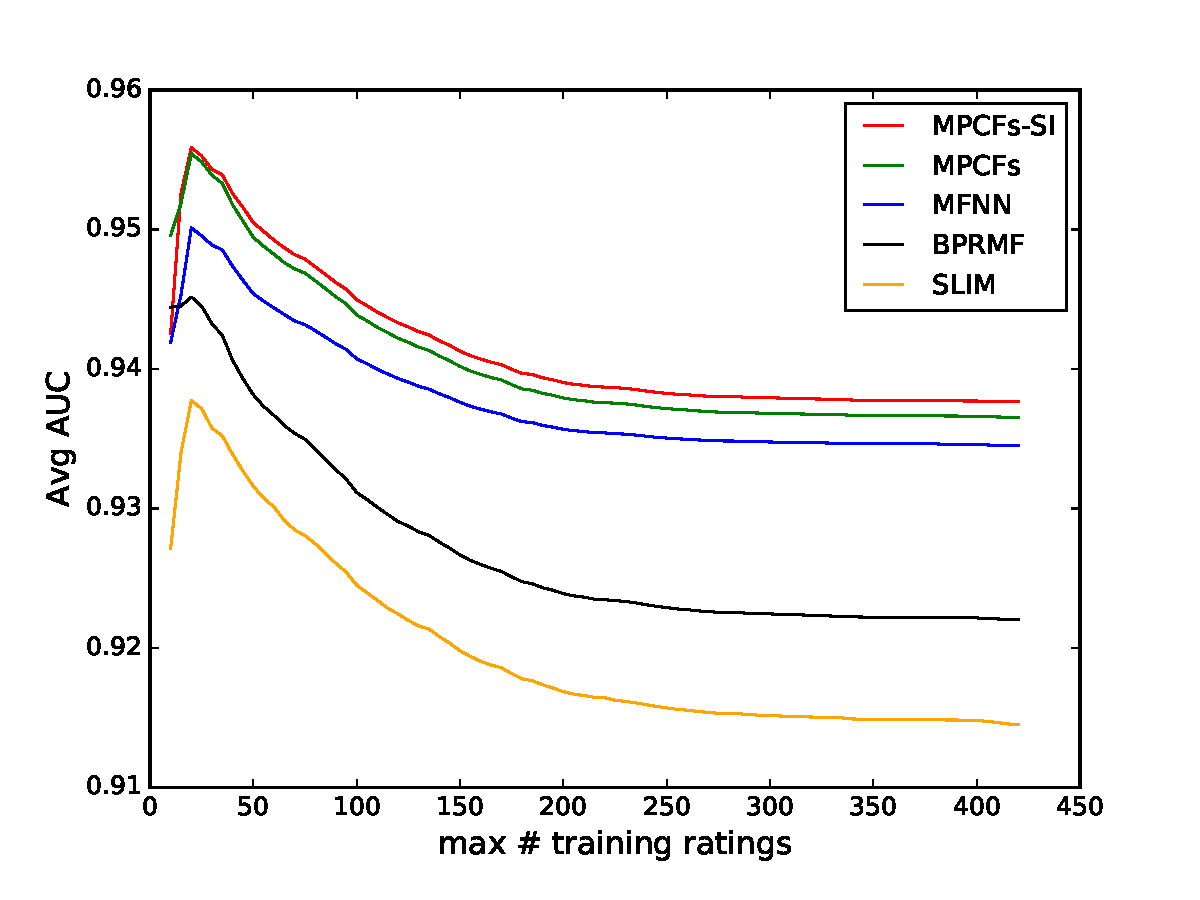
\includegraphics[width=0.7\linewidth]{./section-chapter2/figures/ml-100k_comparison_auc.pdf}
	\caption{Average AUC for a group of users as users with more training ratings were included into that group.
		The performance is measured on the ML-100k-sub dataset.}
	\label{f:ml-100k-comp-auc}
\end{figure}

\begin{figure}[p]
	\centering
	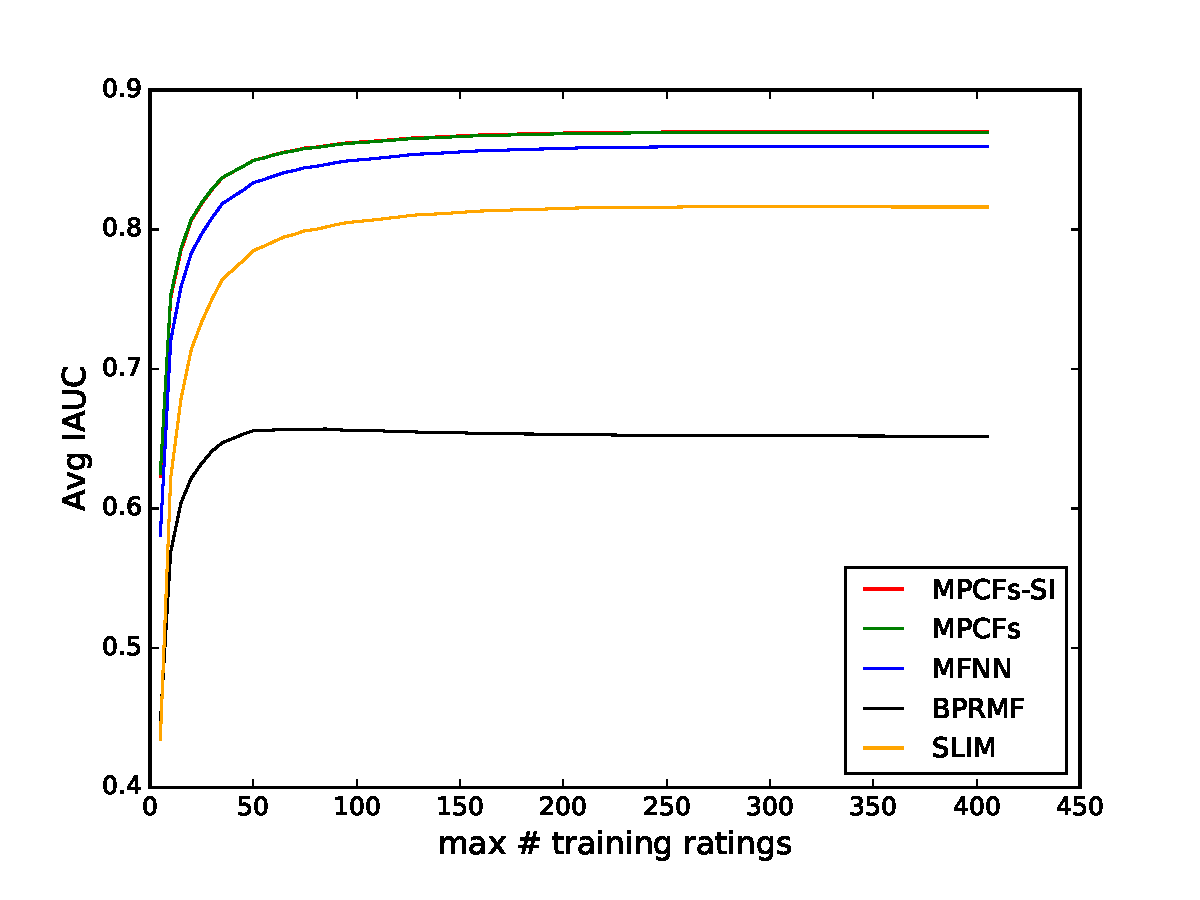
\includegraphics[width=0.7\linewidth]{./section-chapter2/figures/ml-100k_comparison_iauc.pdf}
	\caption{Average IAUC for a group of users as users with more training ratings were included into that group.
		The performance is measured on the ML-100k-sub dataset.}
	\label{f:ml-100k-comp-iauc}
\end{figure}

\begin{figure}
	\centering
	\begin{subfigure}[b]{0.46\linewidth}
		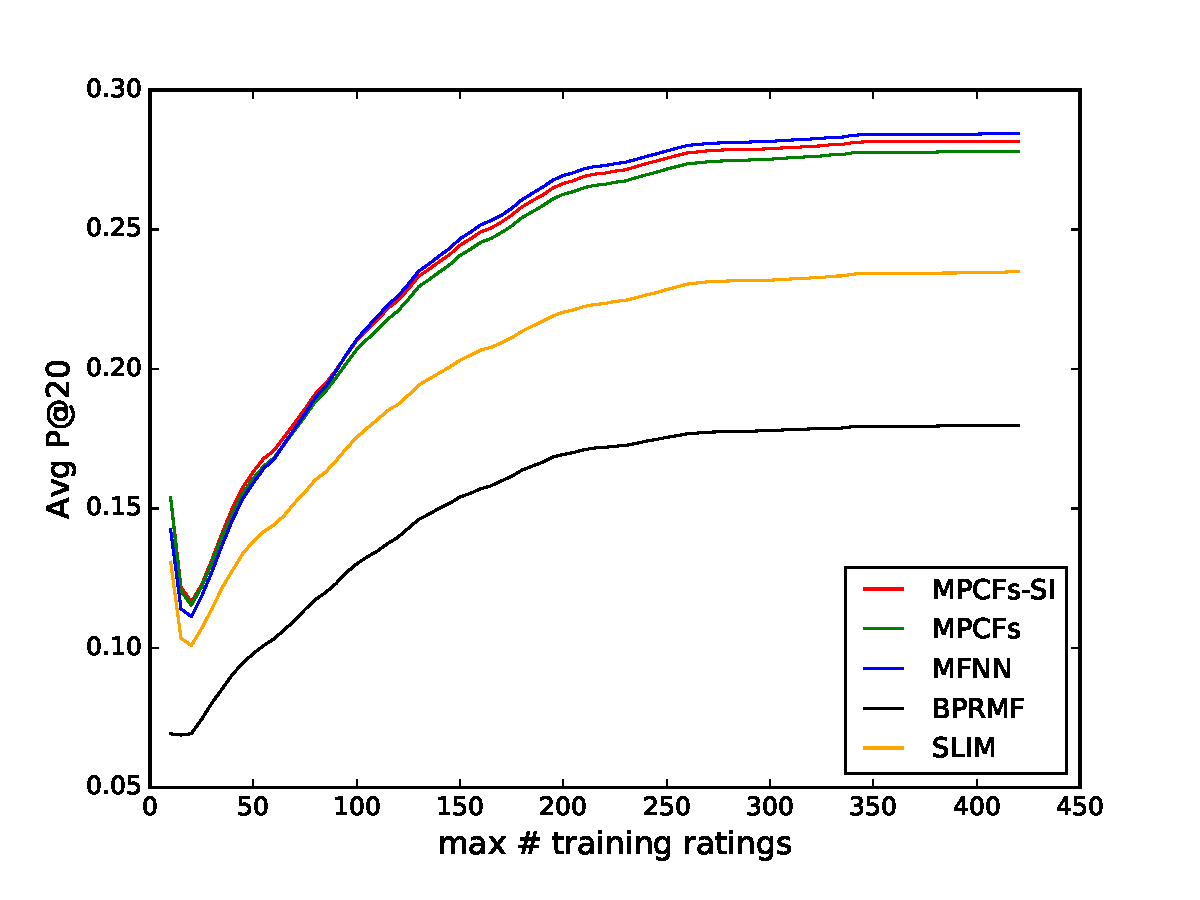
\includegraphics[width=\linewidth]{./section-chapter2/figures/ml-100k_comparison_p20.pdf}
	\end{subfigure}
	\begin{subfigure}[b]{0.46\linewidth}
		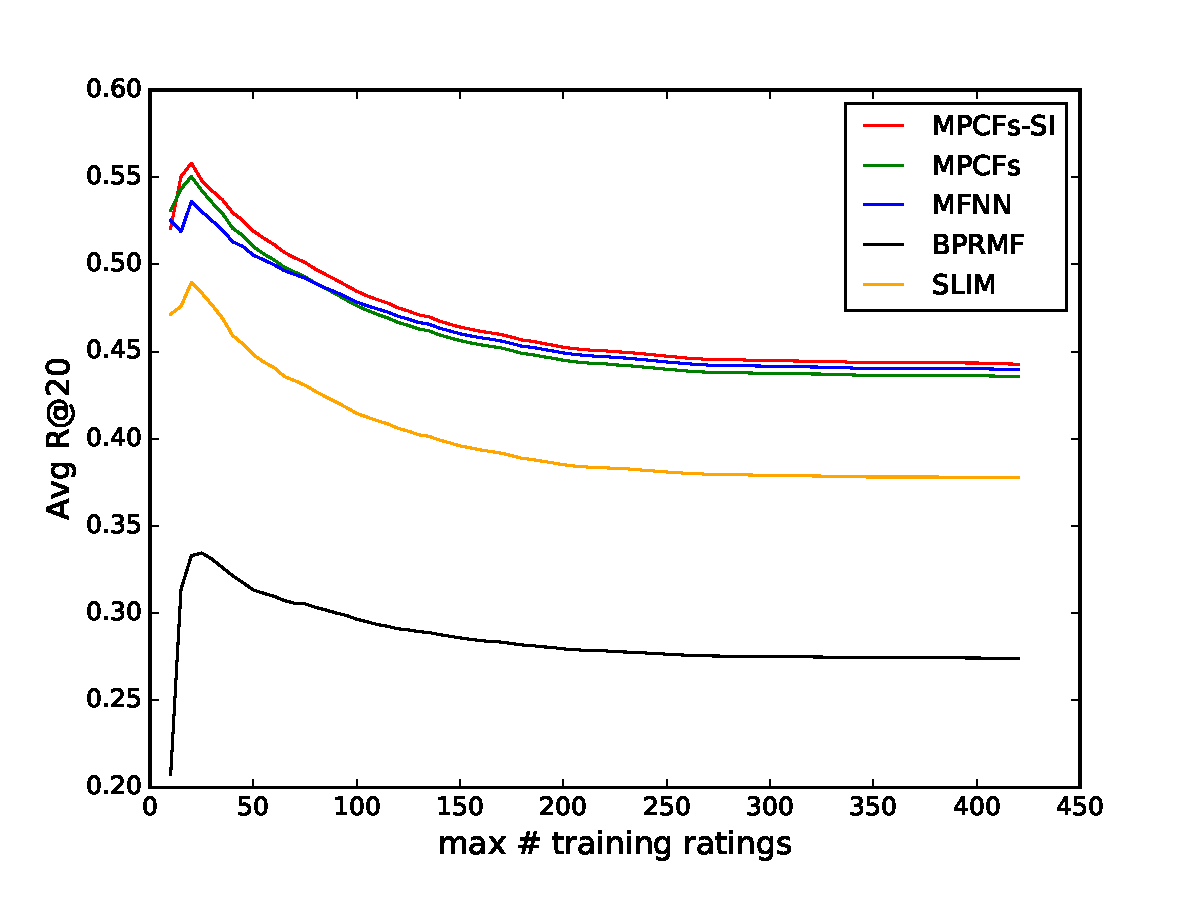
\includegraphics[width=\linewidth]{./section-chapter2/figures/ml-100k_comparison_r20.pdf}
	\end{subfigure}
	\begin{subfigure}[b]{0.46\linewidth}
		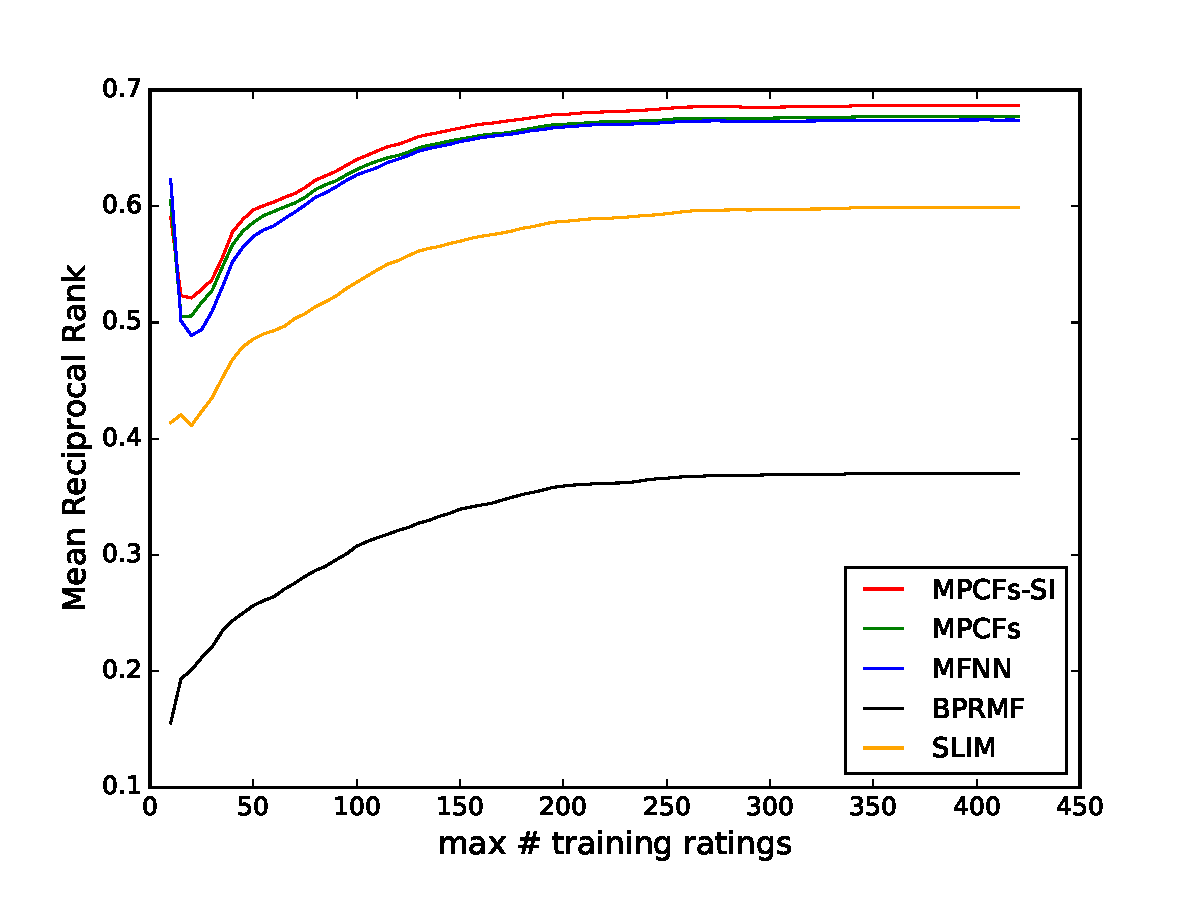
\includegraphics[width=\linewidth]{./section-chapter2/figures/ml-100k_comparison_mrr.pdf}
	\end{subfigure}
	\begin{subfigure}[b]{0.46\linewidth}
		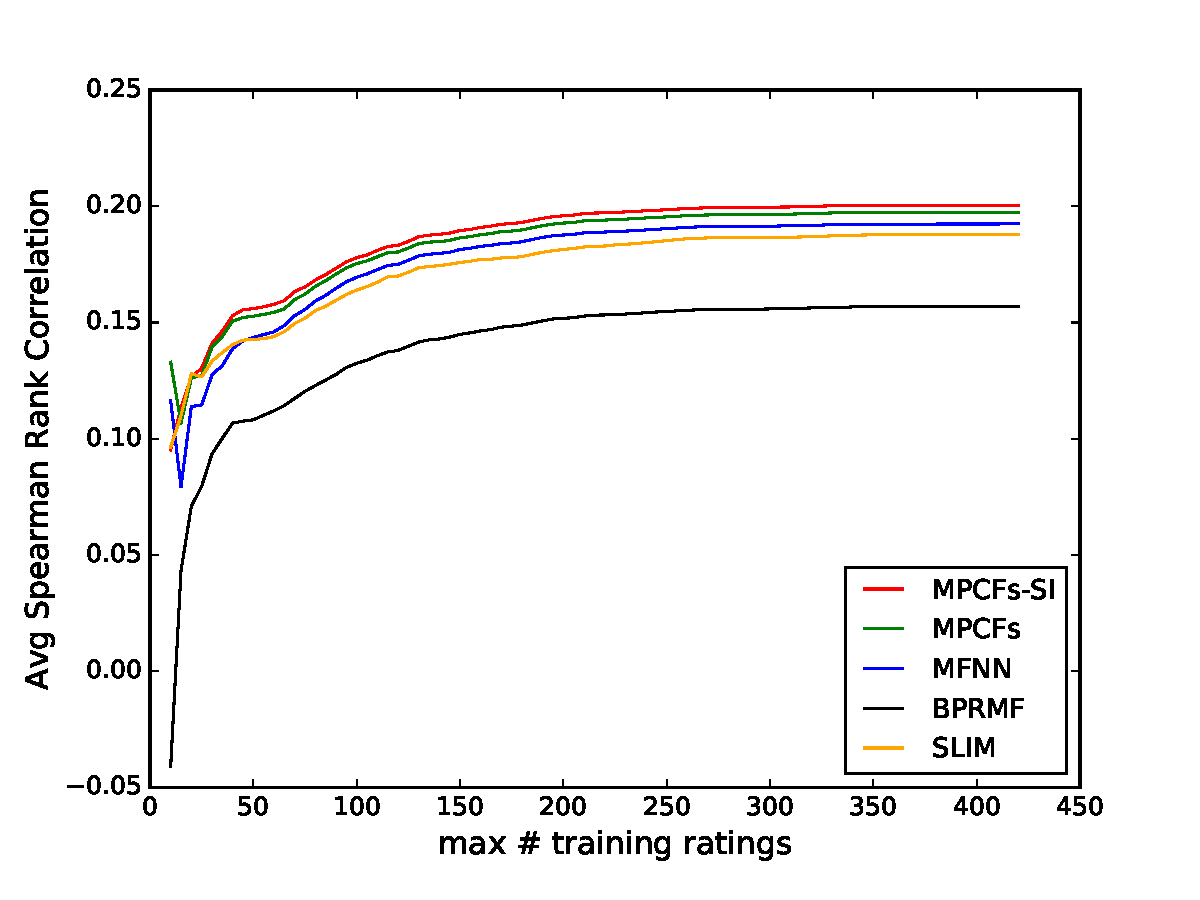
\includegraphics[width=\linewidth]{./section-chapter2/figures/ml-100k_comparison_src.pdf}
	\end{subfigure}
	
	\caption{Measured on the ML-100k-sub dataset.}
	\label{f:ml-100k-comp-group}
\end{figure}


\begin{figure}[p]
	\centering
	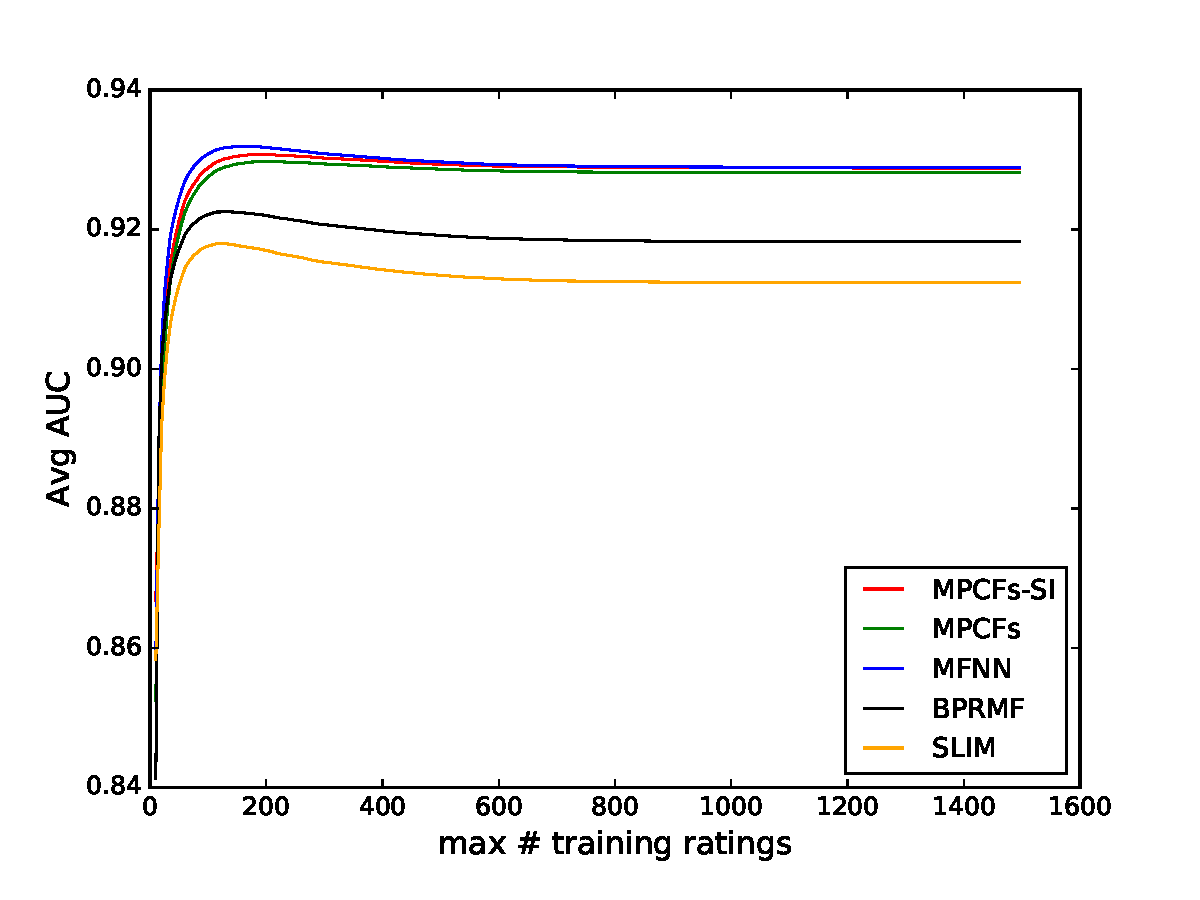
\includegraphics[width=0.7\linewidth]{./section-chapter2/figures/ml-1m_comparison_auc.pdf}
	\caption{
		Average AUC for a group of users as users with more training ratings were included into that group.
		The performance is measured on the ML-1M-sub dataset.}
	\label{f:ml-1m-comp-auc}
\end{figure}

\begin{figure}[p]
	\centering
	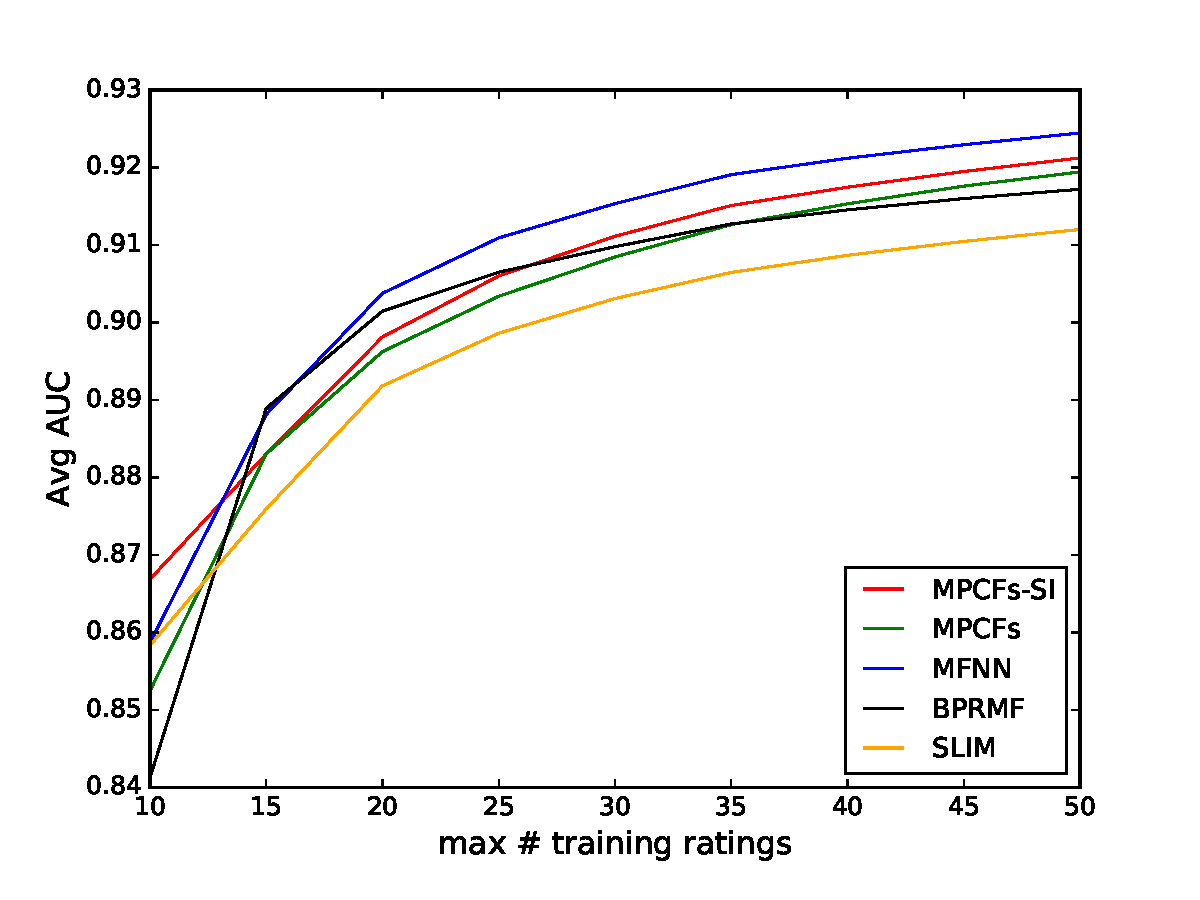
\includegraphics[width=0.7\linewidth]{./section-chapter2/figures/ml-1m_comparison_auc_zoom.pdf}
	\caption{Average AUC for a group of users as users with more training ratings were included into that group.
		The performance is measured on the ML-1M-sub dataset.
		Zoomed version of Figure \ref{f:ml-1m-comp-auc}.}
	\label{f:ml-1m-comp-auc-zoom}
\end{figure}

\begin{figure}[p]
	\centering
	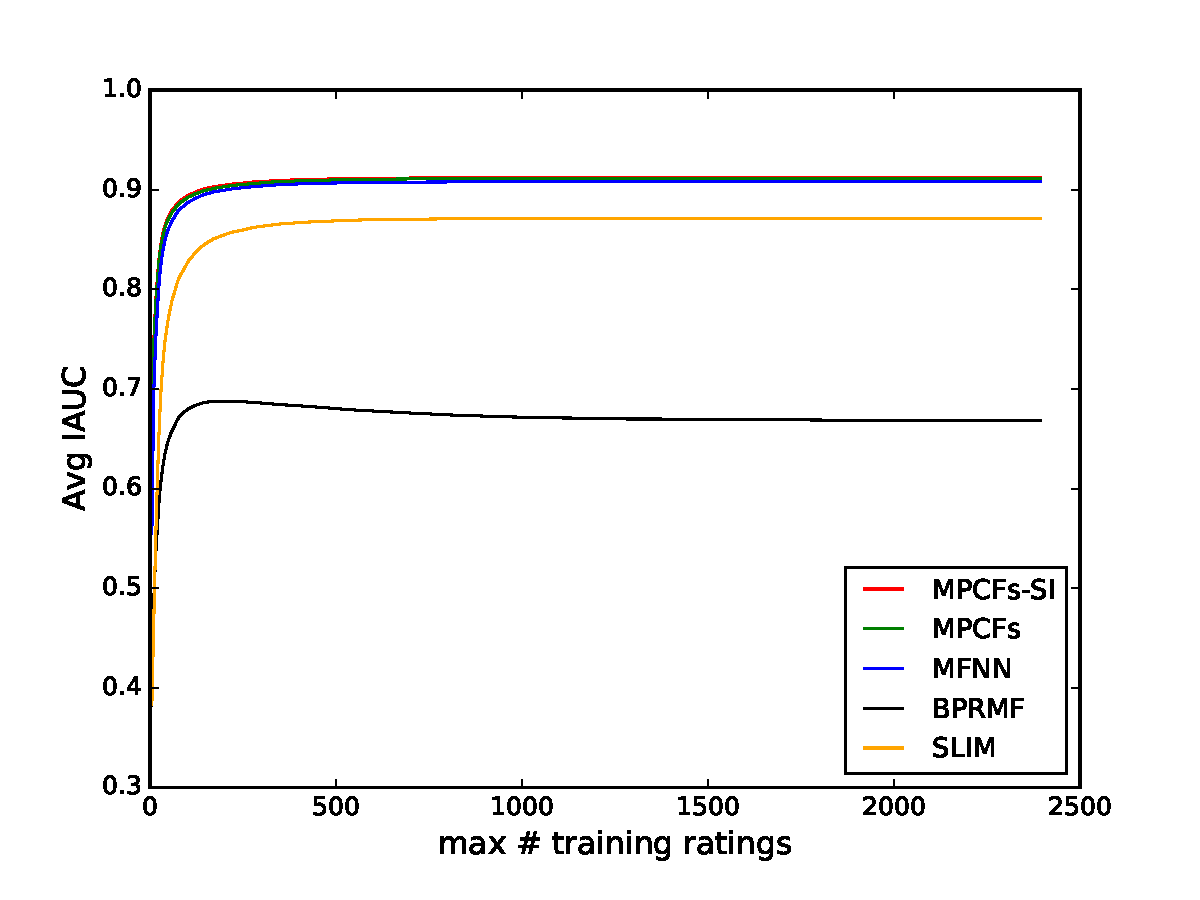
\includegraphics[width=0.7\linewidth]{./section-chapter2/figures/ml-1m_comparison_iauc.pdf}
	\caption{
		Average IAUC for a group of users as users with more training ratings were included into that group.
		The performance is measured on the ML-1M-sub dataset.}
	\label{f:ml-1m-comp-iauc}
\end{figure}

\begin{figure}
	\centering
	\begin{subfigure}[b]{0.46\linewidth}
		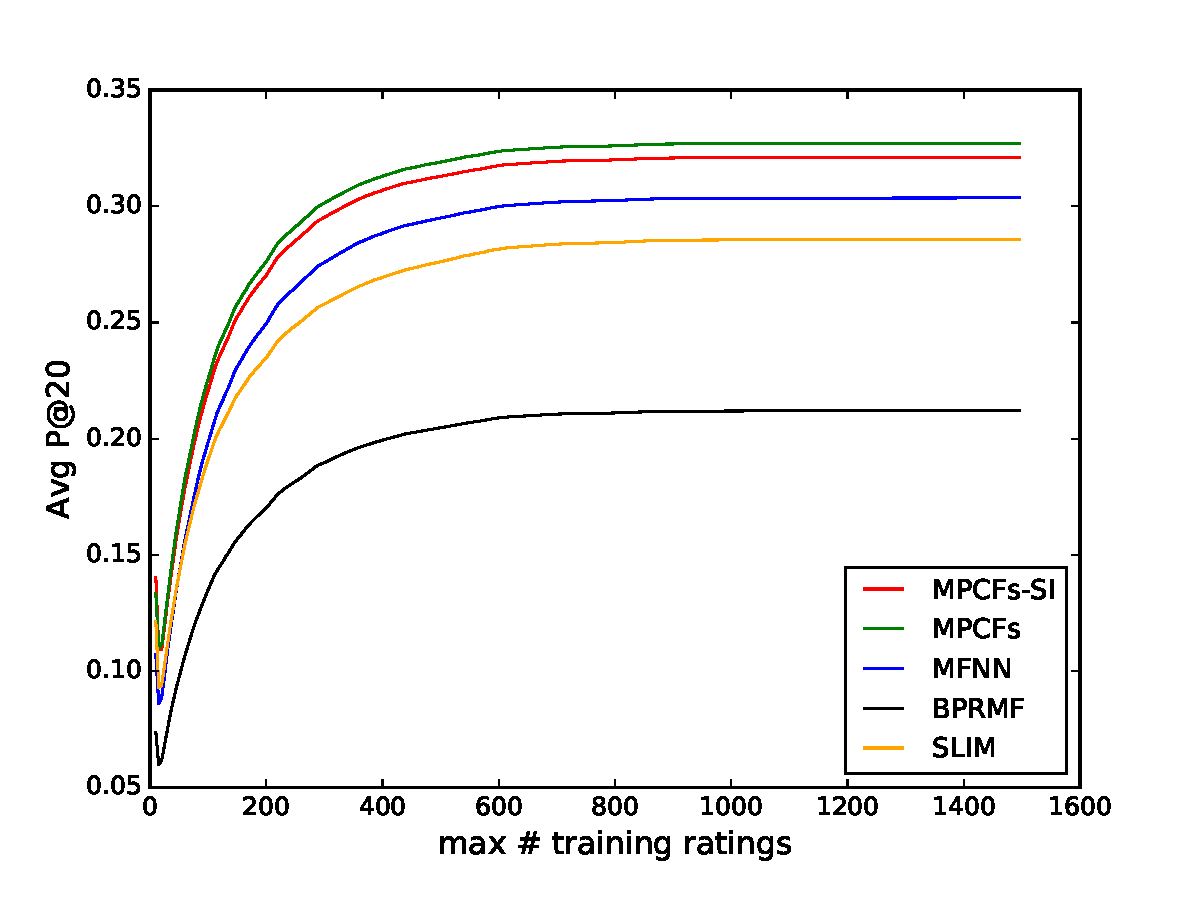
\includegraphics[width=\linewidth]{./section-chapter2/figures/ml-1m_comparison_p20.pdf}
	\end{subfigure}
	\begin{subfigure}[b]{0.46\linewidth}
		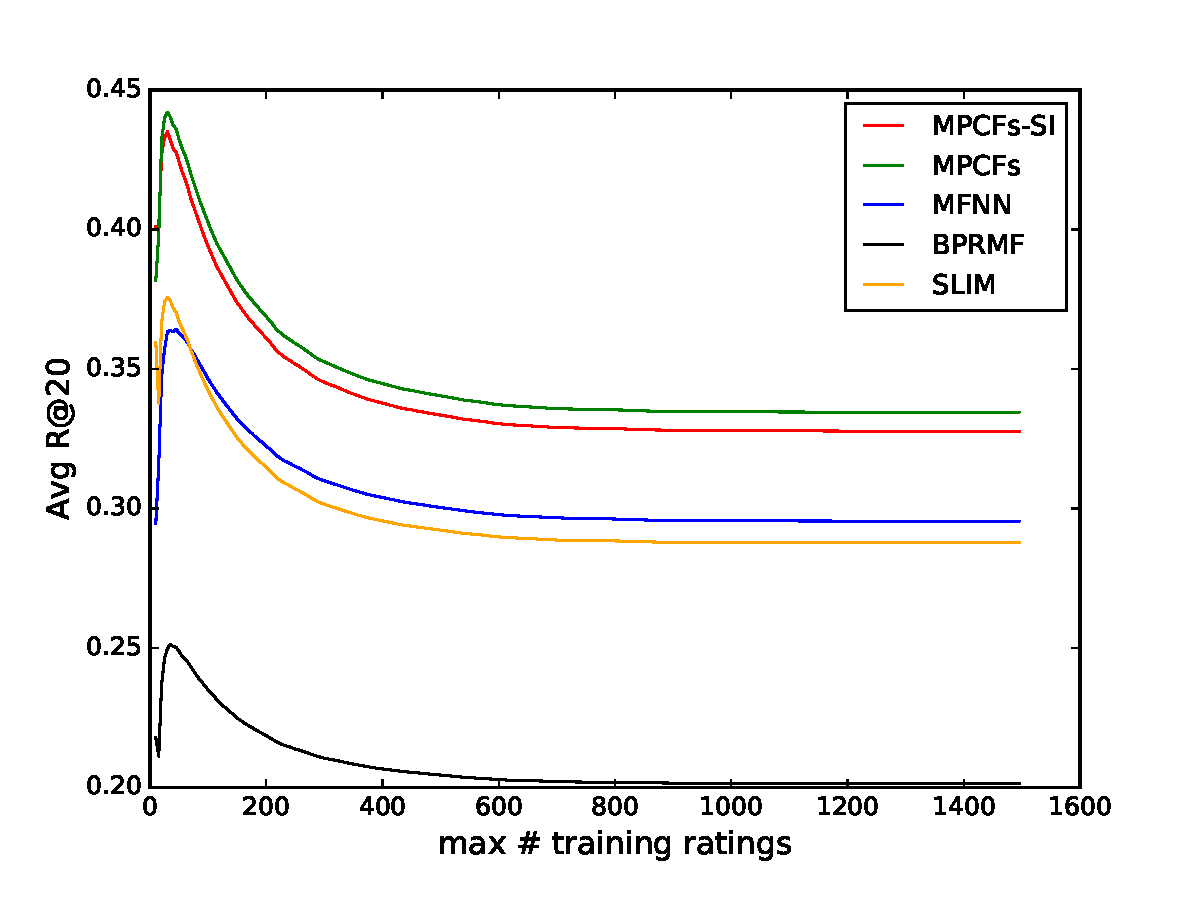
\includegraphics[width=\linewidth]{./section-chapter2/figures/ml-1m_comparison_r20.pdf}
	\end{subfigure}
	\begin{subfigure}[b]{0.46\linewidth}
		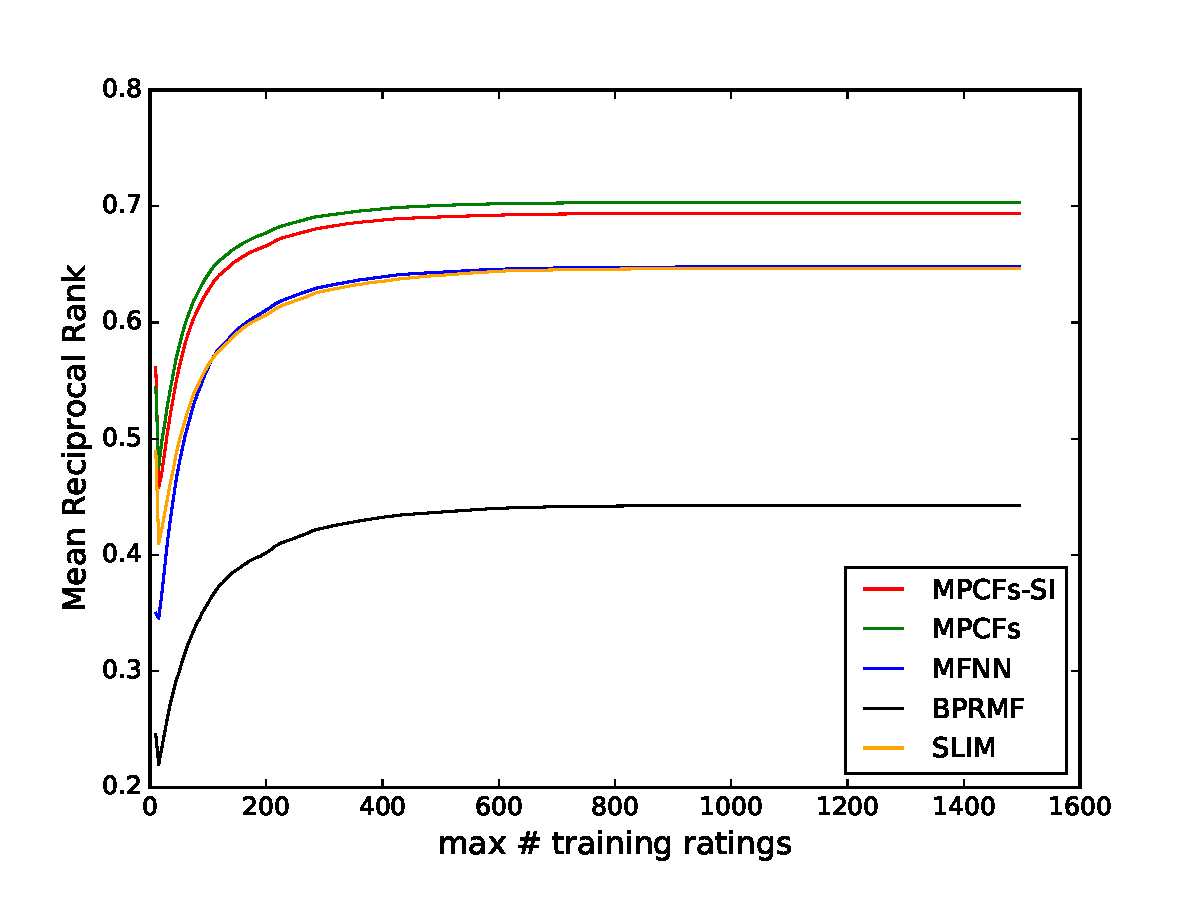
\includegraphics[width=\linewidth]{./section-chapter2/figures/ml-1m_comparison_mrr.pdf}
	\end{subfigure}
	\begin{subfigure}[b]{0.46\linewidth}
		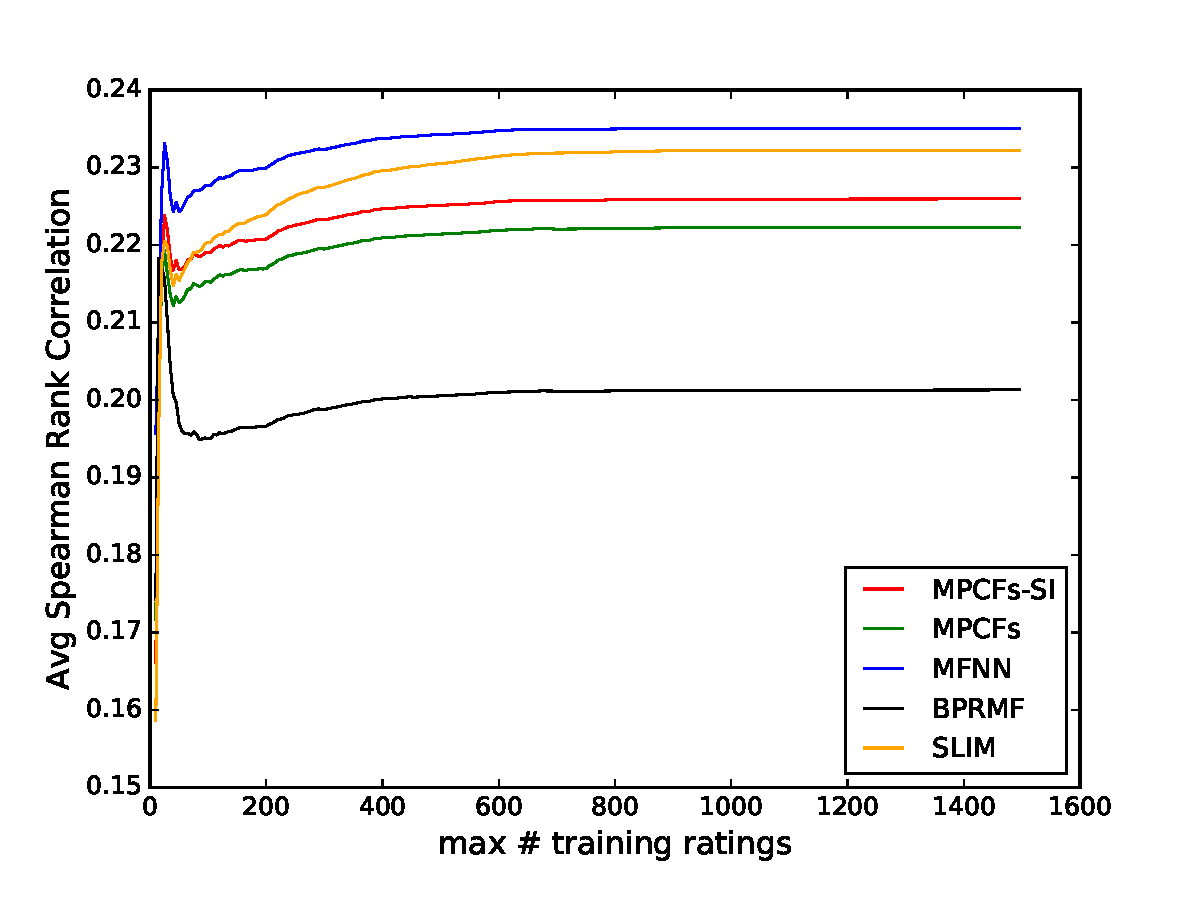
\includegraphics[width=\linewidth]{./section-chapter2/figures/ml-1m_comparison_src.pdf}
	\end{subfigure}
	
	\caption{Measured on the ML-1M-sub dataset.}
	\label{f:ml-1m-comp-group}
\end{figure}
\newpage
\section{System Setup}
\label{st:system-setup} 

A custom software was built in Python.
Our two models, MPCFs-SI and MFNN, as well as the baseline recommender MPCFs \cite{Kabbur2015} and BPRMF \cite{Rendle2009} were implemented by us.
For the baseline recommender SLIM \cite{Ning2011}, we were able to use parts of an open source implementation by Mendeley\footnote{Mendeley mrec - https://github.com/Mendeley/mrec}.
Data handling was done with the Pandas library\footnote{Pandas - http://pandas.pydata.org/} and we have used Numpy\footnote{Numpy - http://www.numpy.org/} for linear algebra operations.
As explained in Section \ref{sst:feature-extraction}, feature vectors for the movies were extracted from their subtitles with the help of Gensim\footnote{Gensim - https://radimrehurek.com/gensim/} and NLTK\footnote{NLTK - http://www.nltk.org/}.
The affine transformation of the MPCFs-SI model, as well as the neural network of the MFNN model, were implemented with Lasagne\footnote{Lasagne - https://github.com/Lasagne/Lasagne} and Theano\footnote{Theano - http://deeplearning.net/software/theano/}.
The source code for this work can be downloaded under https://github.com/marcuniq/bsc-thesis.

\chapter{Conclusions}
\label{c:conclusions}

In this work we have developed two models (MPCFs-SI and MFNN) which incorporate feature vectors of side information in order to improve top-N recommendations.
While similar approaches like \cite{Bao2014} and \cite{Almahairi2015} have shown improvement in rating prediction on almost all of their datasets, we were able to outperform the baseline recommender MPCFs on top-N recommendations only slightly on our two MovieLens datasets.
Our second model MFNN always performed worse than the baseline recommender.

The learning scheme we employed consisted of two steps: first extract feature vectors from movie subtitles via the well established algorithm of Paragraph Vectors\\ \cite{Le2014a}, then using those feature vectors in our models.
Future research efforts should attempt to fully joint learn a matrix factorization model and a movie subtitle model.

% *************** Bibliography ***************
\bibliographystyle{apalike}
\bibliography{C:/Users/Marco/Documents/MendeleyBibtex/BSc-Thesis}

% *************** Appendixes ***************
\appendix
\chapter{Appendix}
\label{a:appendix}

\section{Parameters}
\label{a:best-params}

\subsection{Doc2Vec}
\label{a:doc2vec}
distributed memory: 0 (= distributed bag-of-words: 1), size: 50, hierarchical sampling: 0, negative sampling factor: 5, window: 8, minimum word count: 2, number of epochs: 20, alpha: 0.025, minimum alpha: 0.025, alpha decay: 0.0005

\subsection{MPCFs-SI}
\subsubsection{ML-100k-sub}
Matrix factorization model:\\
learning rate: 0.01, learning rate decay: 0.02, number of epochs: 20, number of latent factors $k$: 128, number of user local preferences $T$: 4, regularization parameter $\lambda_{reg}$: 0.01, zero sample factor: 5\\
Doc2Vec prediction model:\\
learning rate: 0.03, learning rate decay: 0.02, regularization parameter $\lambda_{reg}$: 0.01, balancing parameter $\lambda_{ed}$: 0.001, balancing parameter $\lambda_{cos}$: 0.7

\subsubsection{ML-1M-sub}
Matrix factorization model:\\
learning rate: 0.03, learning rate decay: 0.02, number of epochs: 20, number of latent factors $k$: 96, number of user local preferences $T$: 2, regularization parameter $\lambda_{reg}$: 0.01, zero sample factor: 5\\
Doc2Vec prediction model:\\
learning rate: 0.03, learning rate decay: 0.02, regularization parameter $\lambda_{reg}$: 0.01, balancing parameter $\lambda_{ed}$: 0.0003, balancing parameter $\lambda_{cos}$: 2

\subsection{MFNN}
\subsubsection{ML-100k-sub}
Matrix factorization model:\\
learning rate: 0.03, learning rate decay: 0.02, number of epochs: 20, number of latent factors $k$: 96, regularization parameter $\lambda_{reg}$: 0.01, zero sample factor: 5 \\
Neural network model:\\
layer dimensions: [242, 16, 8, 1], learning rate: 0.03, learning rate decay: 0.02, regularization parameter $\lambda_{nnreg}$: 0.003


\subsubsection{ML-1M-sub}
Matrix factorization model:\\
learning rate: 0.06, learning rate decay: 0.02, number of epochs: 10, number of latent factors $k$: 96, regularization parameter $\lambda_{reg}$: 0.01, zero sample factor: 5 \\
Neural network model:\\
layer dimensions: [242, 4, 1], learning rate: 0.06, learning rate decay: 0.02, regularization parameter $\lambda_{nnreg}$: 0.01


\subsection{MPCFs}
\subsubsection{ML-100k-sub}
learning rate: 0.01, learning rate decay: 0.02, number of epochs: 20, number of latent factors $k$: 128, number of user local preferences $T$: 4, regularization parameter $\lambda_{reg}$: 0.01, zero sample factor: 5

\subsubsection{ML-1M-sub}
learning rate: 0.03, learning rate decay: 0.02, number of epochs: 20, number of latent factors $k$: 128, number of user local preferences $T$: 2, regularization parameter $\lambda_{reg}$: 0.01, zero sample factor: 5


\subsection{BPRMF}
\subsubsection{ML-100k-sub}
learning rate: 0.03, learning rate decay: 0.02, number of epochs: 20, number of latent factors: 128, regularization parameter: 0.01, triplet sample factor: 5

\subsubsection{ML-1M-sub}
learning rate: 0.03, learning rate decay: 0.02, number of epochs: 20, number of latent factors: 128, regularization parameter: 0.001, triplet sample factor: 5

\subsection{SLIM}
\subsubsection{ML-100k-sub}
number of epochs: 5, fit intercept: false, ignore negative weights: true, $l_1$ regularization: 0.003, $l_2$ regularization: 0.00003

\subsubsection{ML-1M-sub}
number of epochs: 5, fit intercept: true, ignore negative weights: true, $l_1$ regularization: 0.001, $l_2$ regularization: 0.003

% *************** Back matter ***************
\backmatter

\normalfont
\clearpage
\listoffigures

\clearpage
\listoftables


\end{document}